\chapter{Experimental methods and results} 


%----------------------------------------------------------------------------------------

%----------------------------------------------------------------------------------------

To experimentally verify the results described above, we ran more than \textbf{3 billion simulations}, generating approximately \textbf{250GB} of data. The code that used to run the simulation and to extract the statistics is available in Github, see Appendix 1 for more details. The full data is also available, see Appendix 2. 


\section{2D lattice simulation}
\label{sec:2d_lattice_simulation}


We used a $L \times L$ square, periodic lattice, which is topologically equivalent to a torus. Each node has four neighbours: one above it, one to the right, one below, and one to the left. The periodicity is represented by the fact that the right neighbors of the nodes in the rightmost column are the nodes in the leftmost column. Similarly, the left neighbours of the leftmost column are the nodes in the rightmost column, the top neighbours of the topmost row are the nodes in the bottom-most row, and the bottom neighbours of the bottom-most row are nodes in the topmost row.

Each node can be in one of two states: dead or alive. Initially, all nodes are in the alive state. With probability $p$, we change state of each individual node to dead. We then compute and store the set of clusters found in the lattice. A cluster is a set of connected nodes sharing the same state. 

Each cluster can either be a finite or infinite. Since the lattice is periodic, \textbf{a cluster is considered infinite if its 1D extension in either direction is greater than or equal to the size of the lattice $L$}. Otherwise, it is a finite cluster. In other words, we imagine a bounding box around each cluster, and if at least of the dimensions of the box is greater than or equal to $L$, the cluster is infinite. 

We generated around 3000 lattices for each pair $(p, L)$, with $p$ ranging from 0 to 1 (with a higher density near the critical points) and $L$ ranging from 16 to 1024.


\section{Percolation probability}

A lattice has percolated if it contains at least one infinite cluster. For each $(p, L)$, we count the number of percolating lattices and divide by the total number of lattices simulated to compute the percolation probability.

In \autoref{fig:sim_perc_prob_1}, we plot the percolation probability against the occupation probability $p$ for various lattice sizes.


\begin{figure}[H]
  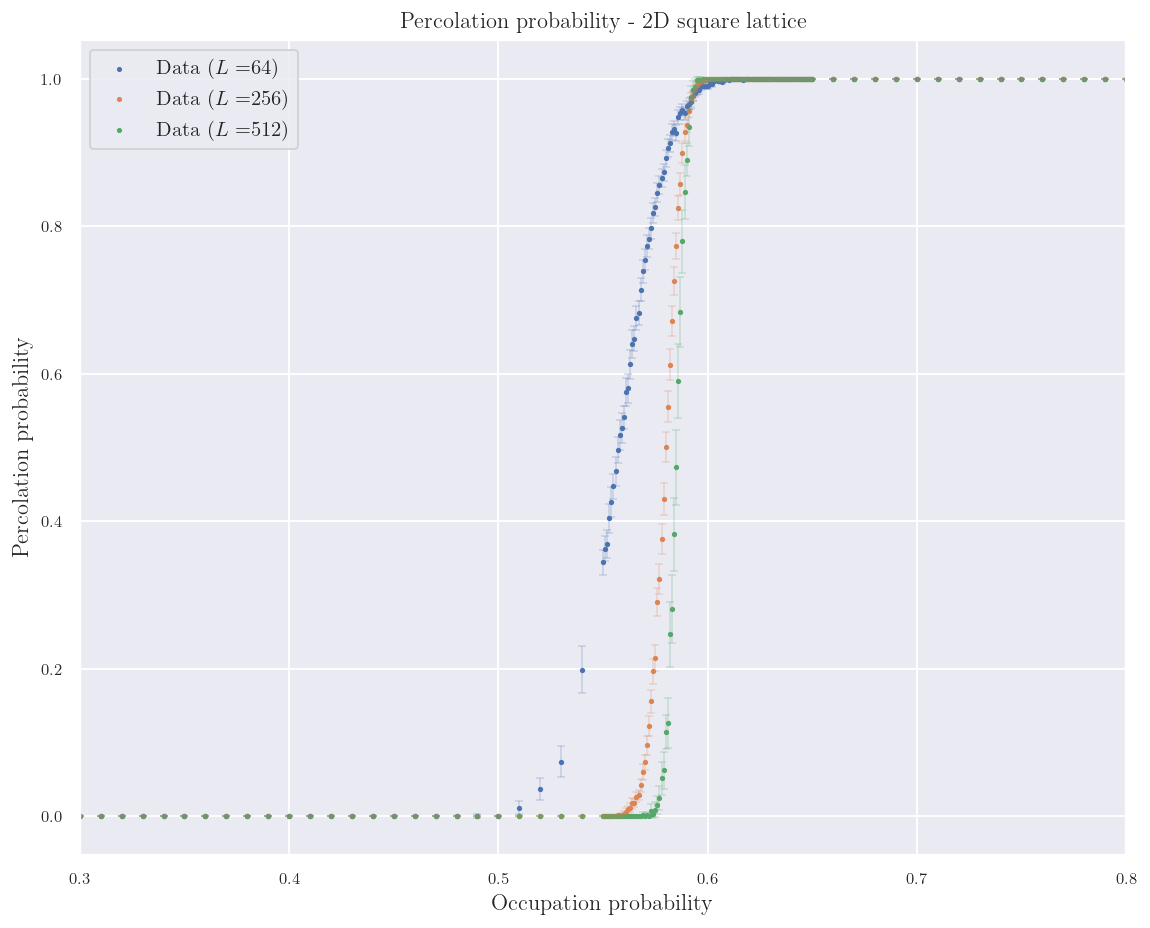
\includegraphics[width=\linewidth]{Images/sim_perc_prob_1.png}
  \caption{Percolation probability curve for various lattice sizes}
  \label{fig:sim_perc_prob_1}
\end{figure}

By visual inspection, we can hypothesize that the curve is a hyperbolic tangent curve: 

$$ 
y(x) = \tanh(x)
$$

We can shift and scale this function so that it's centered at $x=\beta$, and such that it's domain matches our data, i.e. $\mathcal{D}(y) = \left[ 0, 1 \right]$. We'd also like a parameter that controls how steep the transition is between $y=0$ and $y=1$ - this can be done by scaling $x$ by a multiplicative factor $\alpha$. The function becomes

$$ 
y(x) = \frac{\tanh(\alpha(x - \beta)) + 1}{2}
$$ 

In \autoref{fig:sim_perc_prob_2}, we can see the the fitted data points. \autoref{table:sec3_tahn_fit_parameters} contains the precise values.


\begin{figure}[H]
  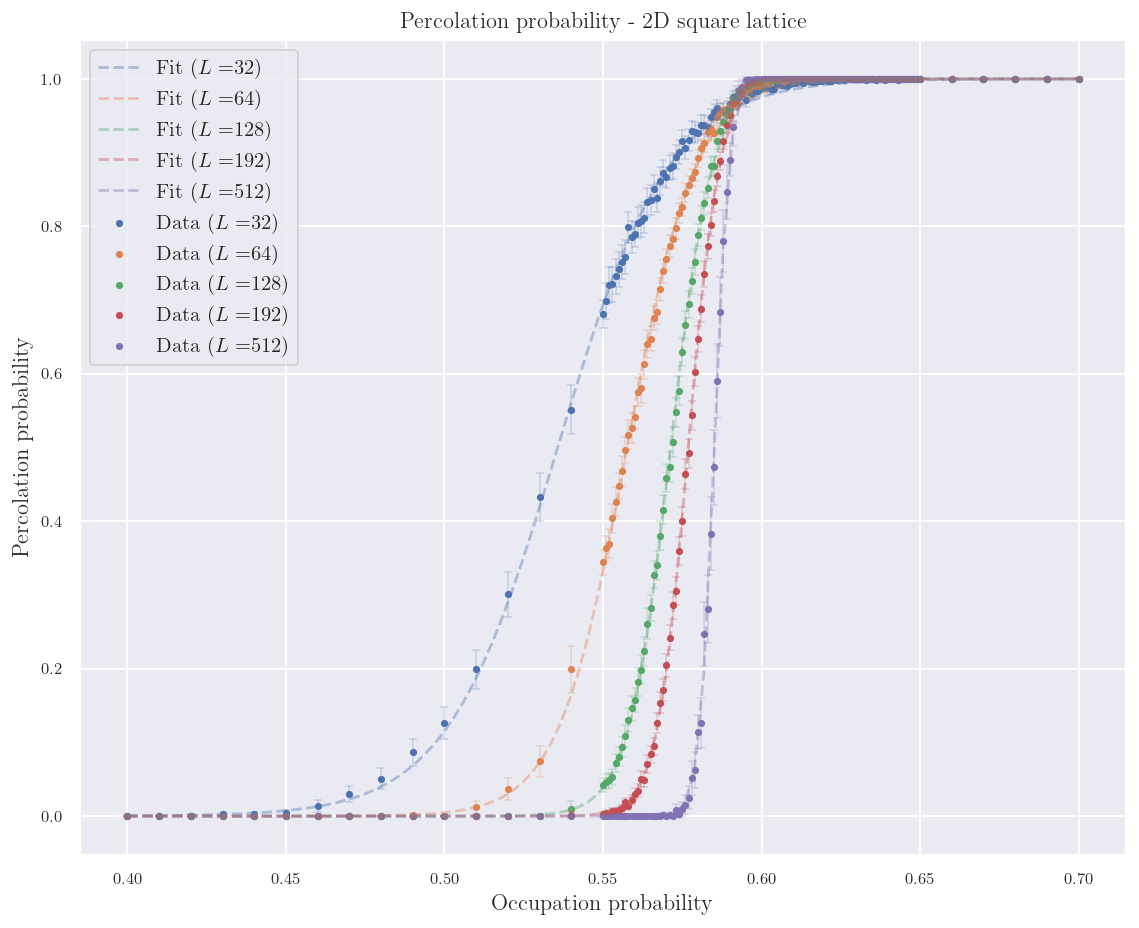
\includegraphics[width=\linewidth]{Images/sim_perc_prob_2.png}
  \caption{Percolation probability with a hyperbolic tangent LMS fit}
  \label{fig:sim_perc_prob_2}
\end{figure}

We notice that the the bigger the lattice, the faster it jumps from $y=0$ to $y=1$. This is consistent with the widely known fact that as L increases, i.e. in the limit $L \rightarrow \infty $, the transition becomes a step function at $p = p_c$. 

Another interesting fact to notice is that with the structure of the function we're fitting, $\beta$ represents the point at which the percolation probability first reaches $\frac{1}{2}$.

These two observations suggest that studying the behaviour of $\alpha$ and $\beta$ as a function of the lattice size $L$ might be interesting. We can see the results obtained in \autoref{fig:sim_perc_prob_param_scaling.png}, in a so called finite-size scaling analysis.

\begin{figure}[H]
  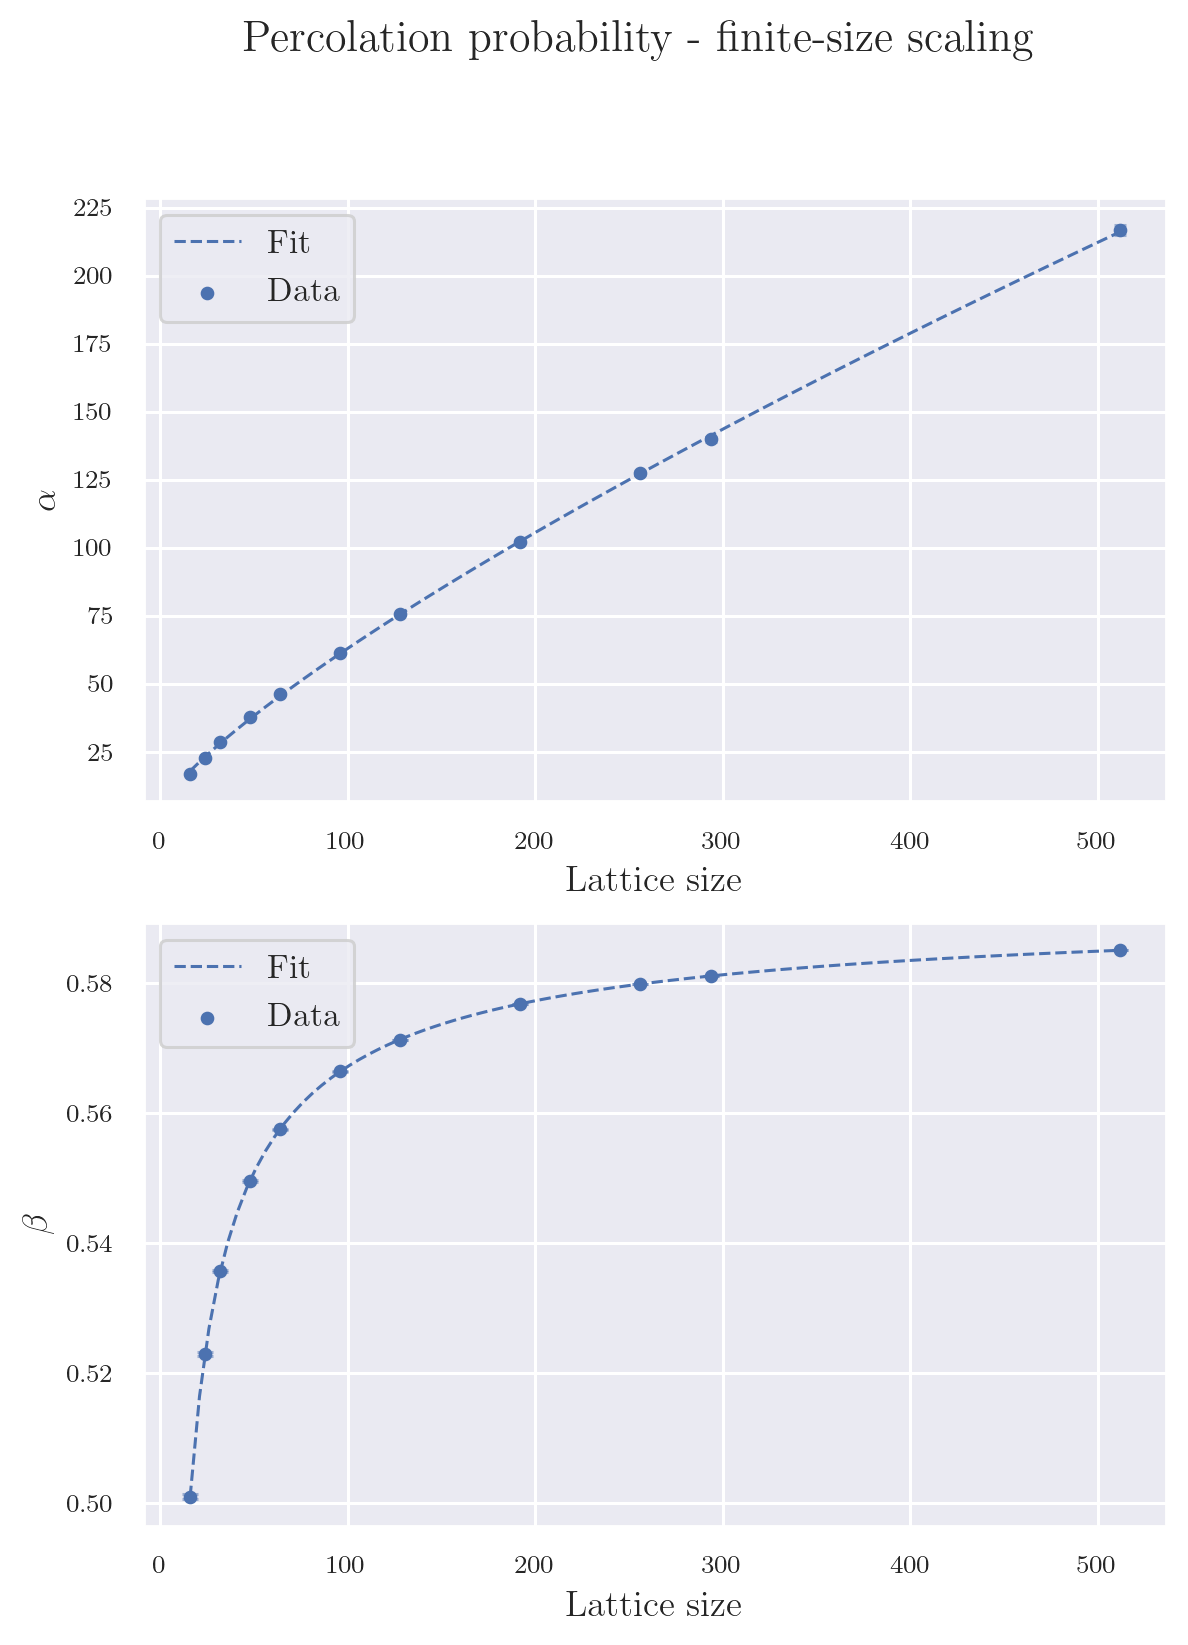
\includegraphics[width=\linewidth]{Images/sim_perc_prob_param_scaling.png}
  \caption{Finite-size scaling analysis of the hyperbolic tangent function}
  \label{fig:sim_perc_prob_param_scaling.png}
\end{figure}

We observe a monotonic growth in $\alpha$ as a function of the lattice size $L$. We were able to get a reasonable fit by using the ansatz

$$ 
    \alpha(L) = a L^n + b
$$

The precise values for the constants $a$, $n$ an $b$ can be seen in \autoref{table:pp_slope_finite_size_scaling_params}.

Of course, 
$$ 
\lim_{L\to\infty} a L^n + b = \infty \hspace{0.5cm} a > 0, n>0
$$

Since $\alpha$ controls how steep the hyperbolic tangent curve is, that is, how fast it goes from 0 to 1, this supports the hypothesis that as we increase $L$, the curve gets arbitrarily close to a step function. 


The parameter $\beta$, on the other hand, behaves differently. We were able to get a fairly good fit by using the ansatz 

$$ 
\beta(L) = c - a e^{\frac{L^n}{b}}
$$ 

The precise values for $a$, $n$, $b$ an $c$ can be seen in \autoref{table:pp_center_finite_size_scaling_params}. 

It is clear that 
$$ 
\lim_{L\to\infty} c - a e^{\frac{L^n}{b}} = c
$$

Since $\beta$ represents occupation probability at which the percolation probability reaches 1/2, the limit above allows us to estimate $p_c$, the critical probability of our system - we do so by interpreting $p_c$ as $\beta$ in the limit of an infinite lattice. This value comes out to be $\mathbf{0.5907(2)}$.

\subsection{Errors}

The error estimates for the percolation probability were computed by treating it as a Bernoulli random variable. We used a 99\% confidence interval and the expression 

$$ 
\textrm{Error} = z \sqrt{\frac{\bar{p}(1-\bar{p})}{n}}
$$

where z is the value coming from the z-table for the desired confidence interval (numerically, $z=2.576$), $\bar{p}$ is the mean of the observations, and $n$ is the number of observations.

See (REF) for more information.

\section{Percolating cluster strength}

The percolating cluster strength represents the probability that a randomly picked node belongs to a infinite cluster. This was numerically approximated by counting the number of nodes belonging to the (possibly multiple) infinite clusters and dividing by the total number of nodes. The results obtained can be seen in \autoref{fig:sim_perc_clust_strength_1}.

\begin{figure}[H]
  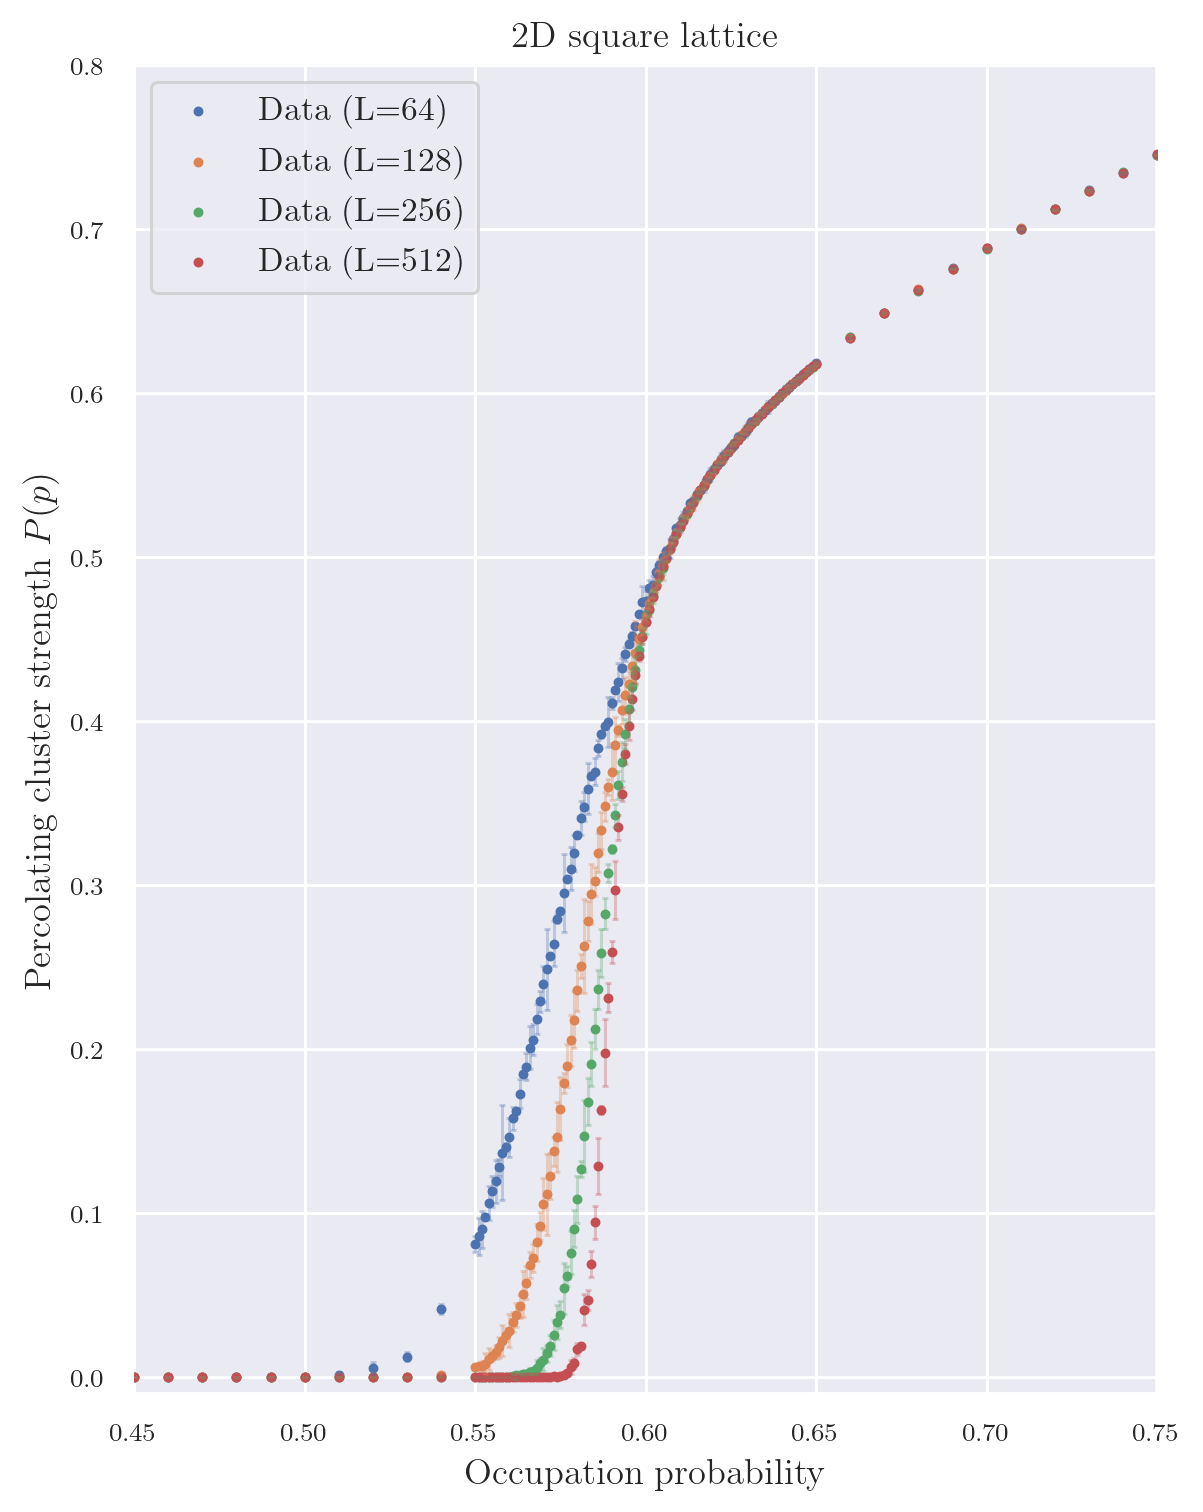
\includegraphics[width=\linewidth]{Images/sim_perc_clust_strength_1.png}
  \caption{Percolating cluster strength versus occupation probability for various lattice sizes.}
  \label{fig:sim_perc_clust_strength_1}
\end{figure}

As discussed in \autoref{sec:th_percolating_cluster_strength}, we expect to see the percolating cluster strength $P(p)$ go from being zero for $p < p_c$ to a non-zero value for $p > p_c$. This is precisely what we see in \autoref{fig:sim_perc_clust_strength_1}. It's also possible to notice that the transition becomes more abrupt for larger lattice sizes, which provides evidence for intuition that this transition approaches a step function as $L \to \infty$.
Unfortunately, we were not able to find an ansatz that approximates this curve well, and therefore can't provide at this time a convincing numerical estimation for the "abruptness" of this transition or how fast it approaches the step function. 


\subsection{Errors}

The errors in the calculation of $P(p)$ were estimated by computing the standard deviation of the sample of values obtained numerically.


\section{Mean cluster size}

The mean cluster size $\chi(p)$ represents the average number of nodes in the finite clusters as defined in \autoref{sec:2d_lattice_simulation}. For each simulation, we loop over the finite clusters, adding their sizes. We then divide the sum by the number of finite clusters to get the average in a particular simulation/lattice. Afterwards, we average again, this time over lattices (of course, this averaging is only done over lattices with the same occupation probability $p$ and size $L$). 

The results can be seen in \autoref{fig:sim_mean_cluster_size_1}.



\begin{figure}[H]
  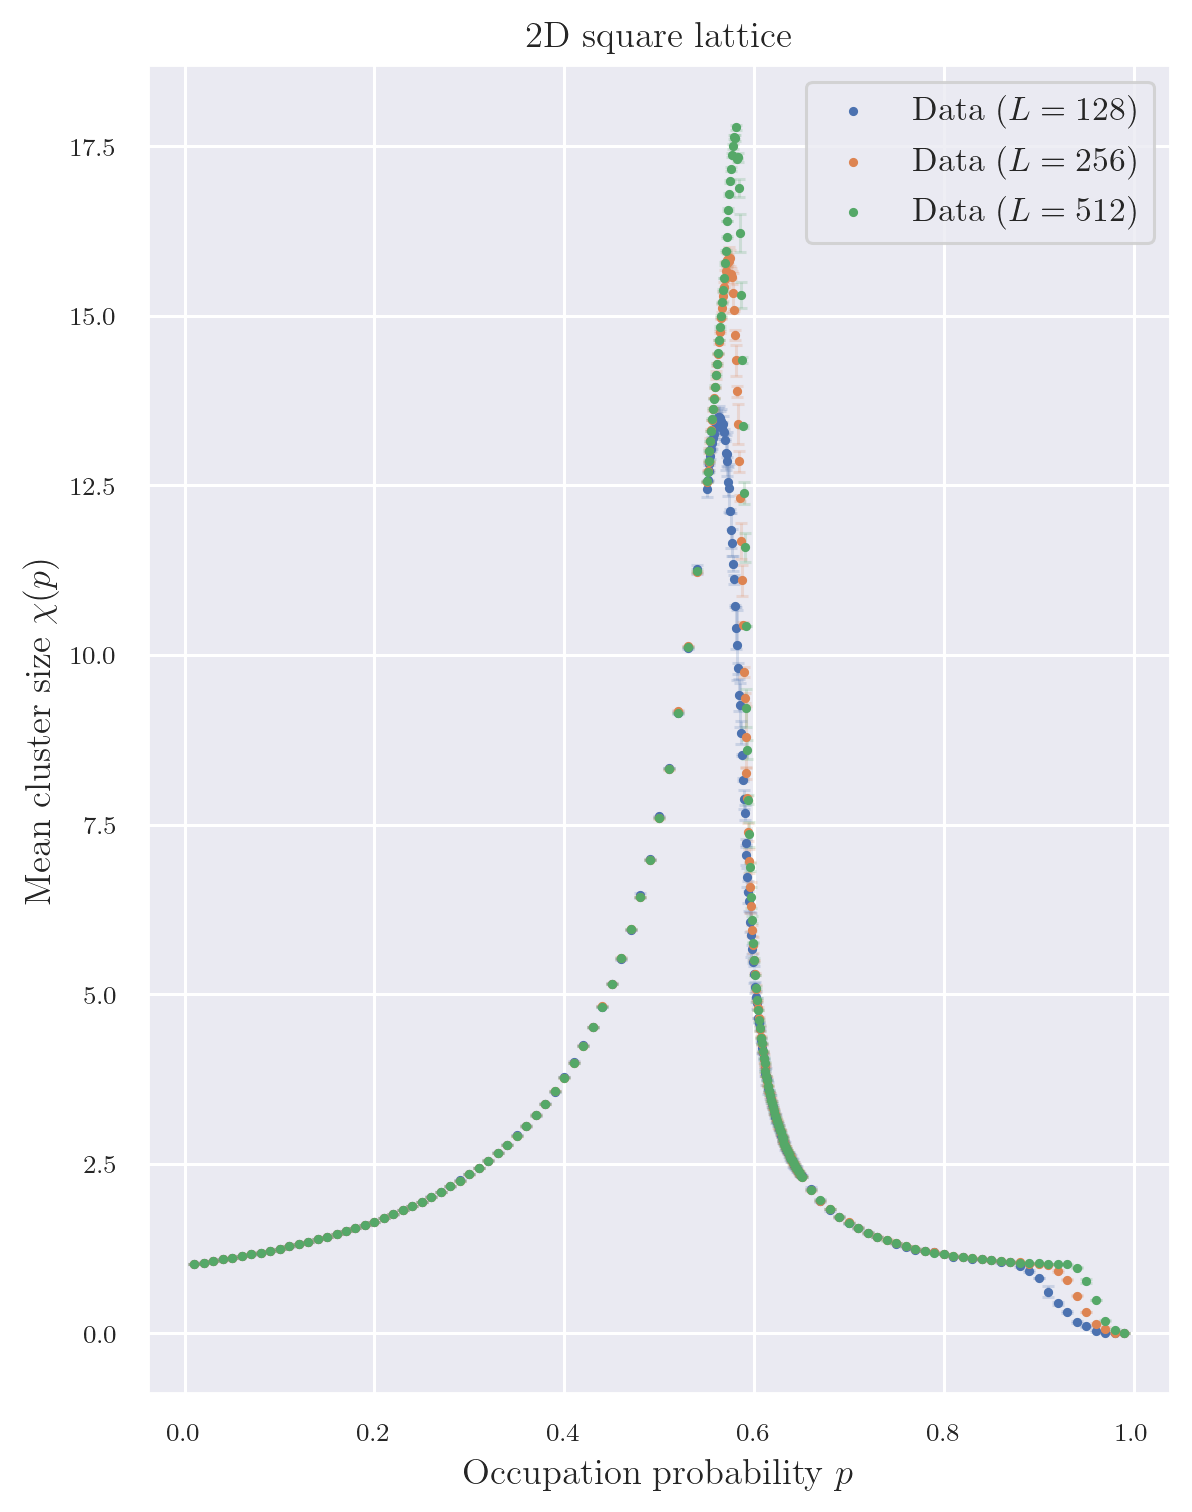
\includegraphics[width=\linewidth]{Images/sim_mean_cluster_size_1.png}
  \caption{Mean finite cluster size versus occupation probability for various lattice sizes}
  \label{fig:sim_mean_cluster_size_1}
\end{figure}


As expected, we see a monotonic increase in $\chi(p)$ up to a maximum value, corresponding to some sort of critical value, and then a somewhat faster, monotonic decrease after the maximum. There is also an interesting kink close to $p=0.9$ which we did not investigate further.
The presence of the peak immediately presents itself as an opportunity to check some of the facts presented in \autoref{sec:th_mean_cluster_size}. 


\autoref{fig:sim_mean_cluster_size_peak_height} shows the peak height $H$ as a function of the lattice size we obtained from our data, and \autoref{table:pp_mean_cluster_size_peak_values} shows the precise values obtained.

\begin{figure}[H]
  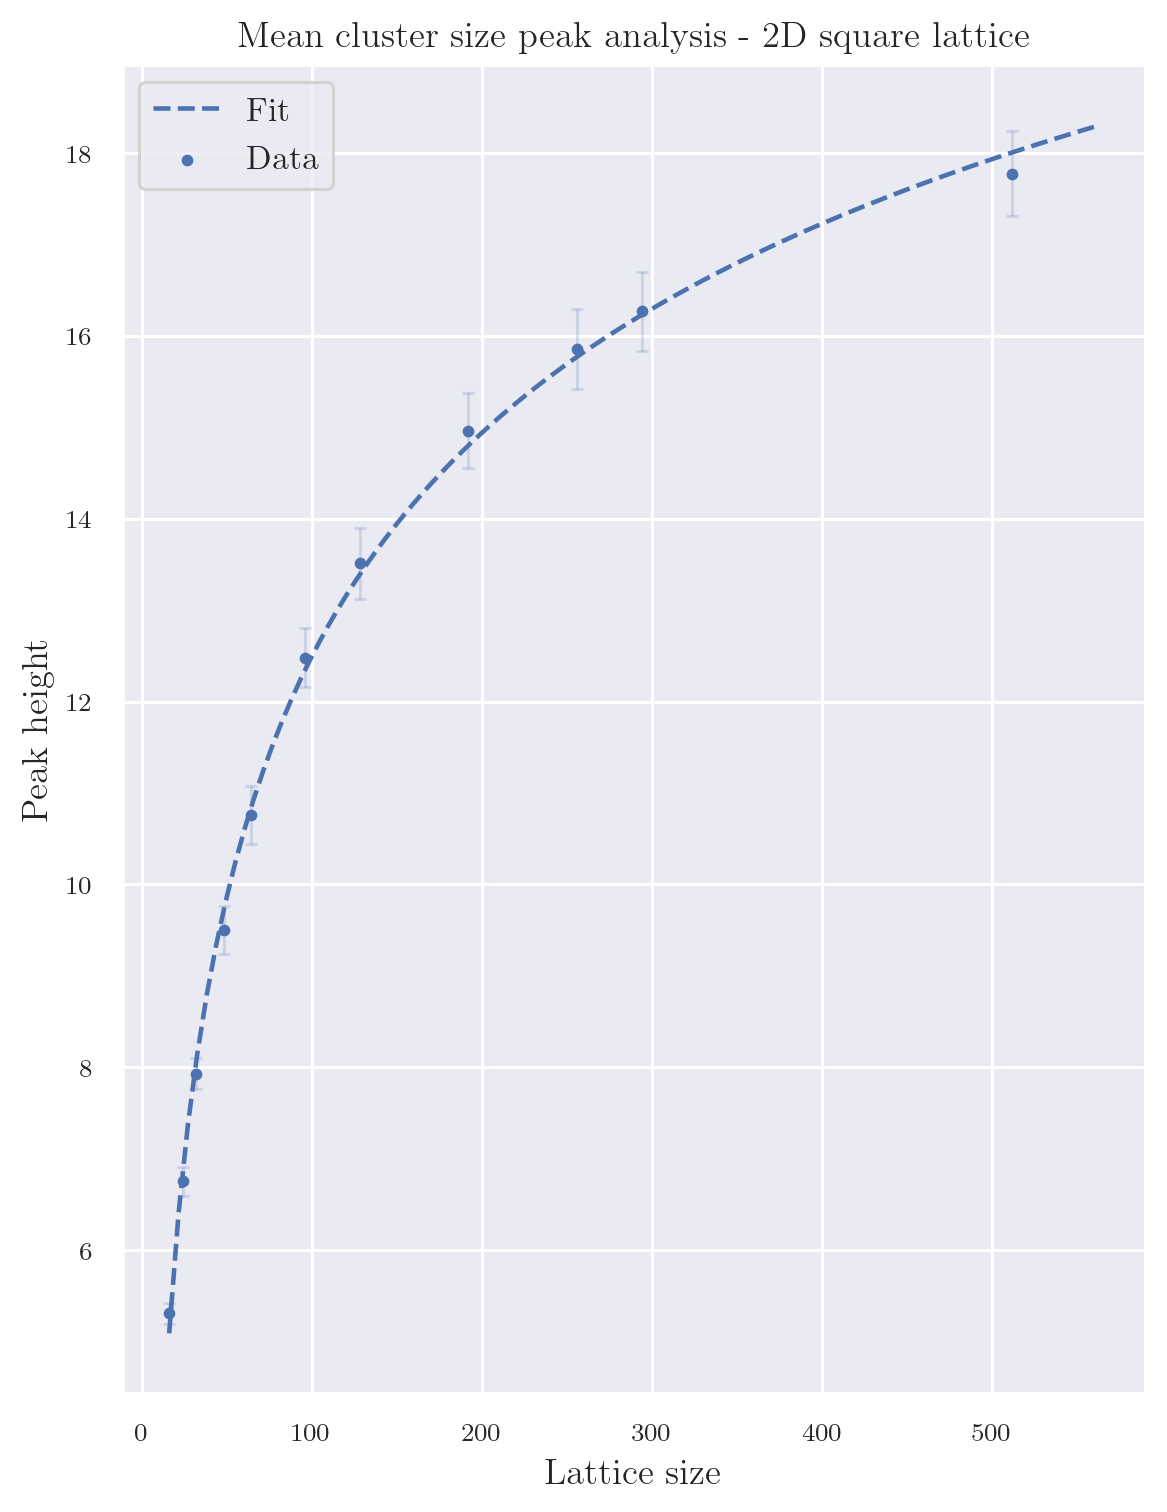
\includegraphics[width=\linewidth]{Images/sim_mean_cluster_size_peak_height.png}
  \caption{Mean cluster size, peak height for various lattice sizes}
  \label{fig:sim_mean_cluster_size_peak_height}
\end{figure}

As expected, the height grows with the lattice size. The ansatz used to fit the curve is
$$ 
H(L) = a \log(bL)^c + d
$$

The precise values of $a$, $b$, $c$ and $d$ can be seen in \autoref{table:pp_mean_cluster_size_peak_height_finite_size_scaling_params}.

Since 
$$
\lim_{L\to\infty} a \log(bL)^c = \infty
$$

This data supports the hypothesis that as we increase $L$, the peaks height does not converge to any finite height, and instead diverges.


Next, we consider the peak position $K$ as a function of the lattice size $L$. While the peak height is expected to diverge, as discussed above, one expects that the peak probability would converge the true percolation threshold $p_c$ as $L$ increases. 
\autoref{fig:sim_mean_cluster_size_peak_position} shows the probability at which the peak is located, $K$, as a function of lattice size, and \autoref{table:pp_mean_cluster_size_peak_positions} shows the numerical values.


\begin{figure}[H]
  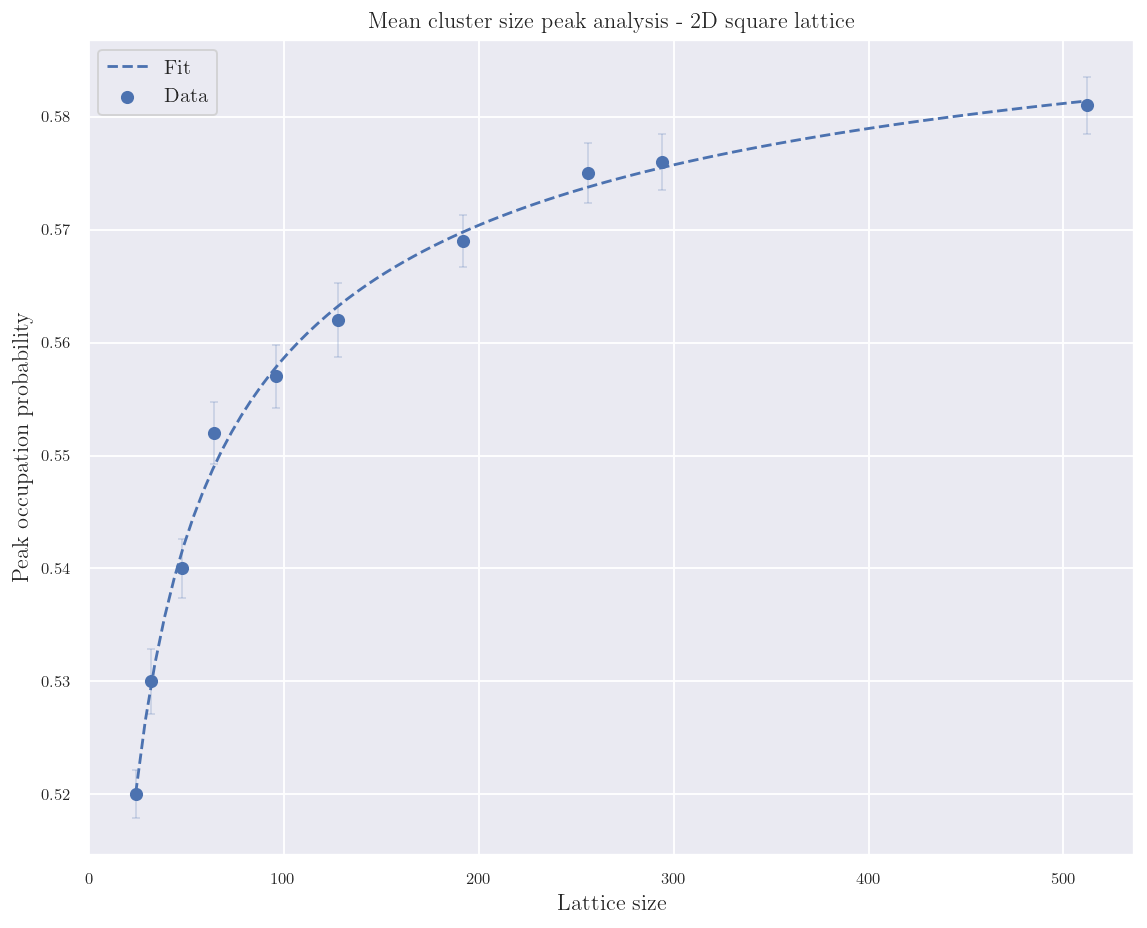
\includegraphics[width=\linewidth]{Images/sim_mean_cluster_size_peak_position.png}
  \caption{Mean cluster size, peak position for various lattice sizes}
  \label{fig:sim_mean_cluster_size_peak_position}
\end{figure}


The ansatz used in the fit above is again

$$ 
    K(L) = c - a e^{\frac{L^n}{b}}
$$

So we conclude that this is, as predicted, evidence for the percolation threshold converging to a finite numerical value (namely, $c$). The precise values for all the fit parameters can be seen in \autoref{table:pp_mean_cluster_size_peak_position_finite_size_scaling_params}. Using this method, we estimate $p_c$ to be \textbf{0.5986(4)}. 

\subsection{Errors}

Again, the errors in the calculation of $\chi(p)$ are estimated by the standard deviation of the sample obtained numerically.

\section{Correlation function and correlation length}



The correlation function was estimated by repeatedly (128000 times) selecting two random nodes from the lattice, computing its distance (we used the Manhattan distance (REF)), and then checking whether they belong to the same finite cluster. Averaging over many lattices, this allows us to to estimate the probability that two nodes at a given distance belong to the same cluster, which is the definition of the correlation function $g(r)$.


\begin{figure}[H]
  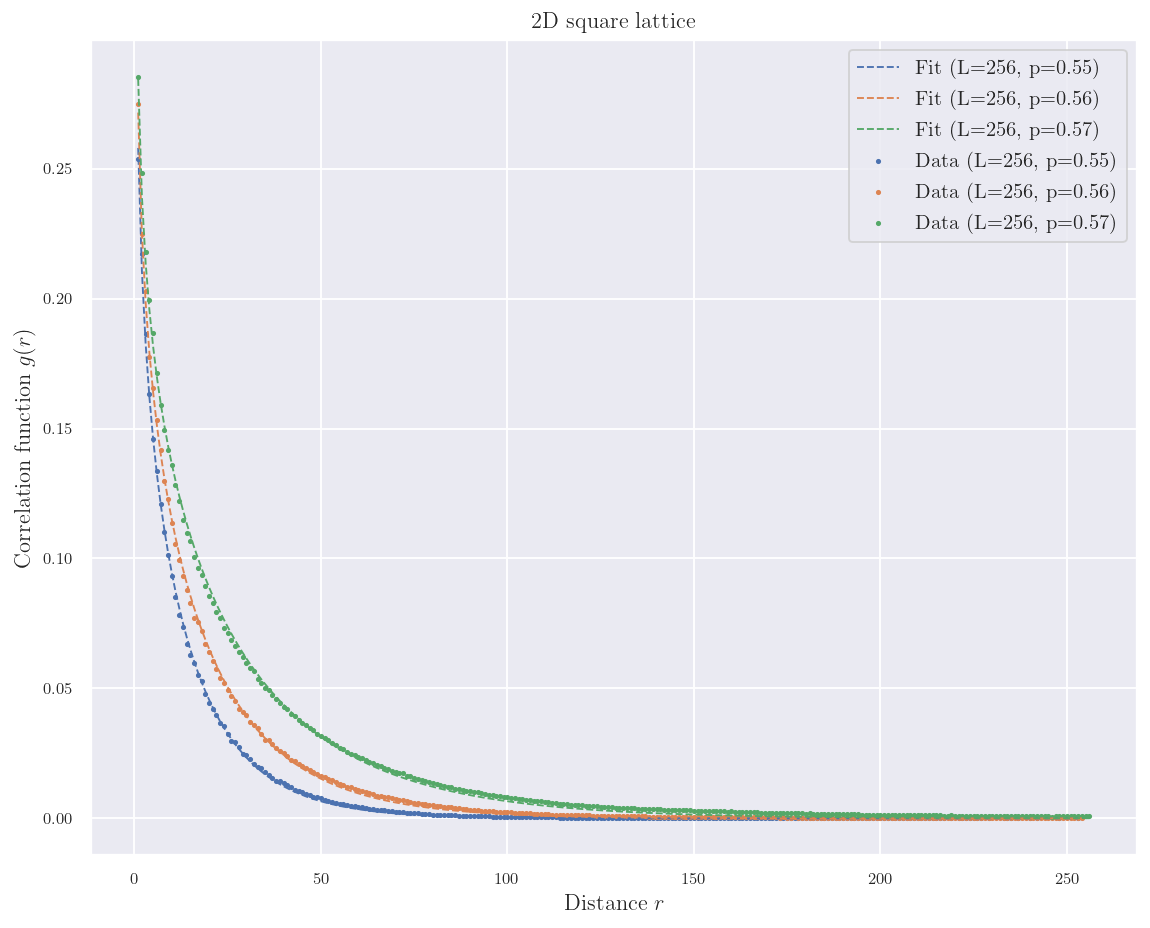
\includegraphics[width=\linewidth]{Images/sec3_corr_func_1.png}
  \caption{Correlation function for various sizes and occupation probabilities}
  \label{fig:sec3_corr_func_1}
\end{figure}


To estimate the correlation length $\xi$, we fitted the data obtained above to the function below

$$ 
 g(r) \propto r^{-\nu} e^{-\frac{r}{\xi}}
$$ 

This gives us the plot below

\begin{figure}[H]
  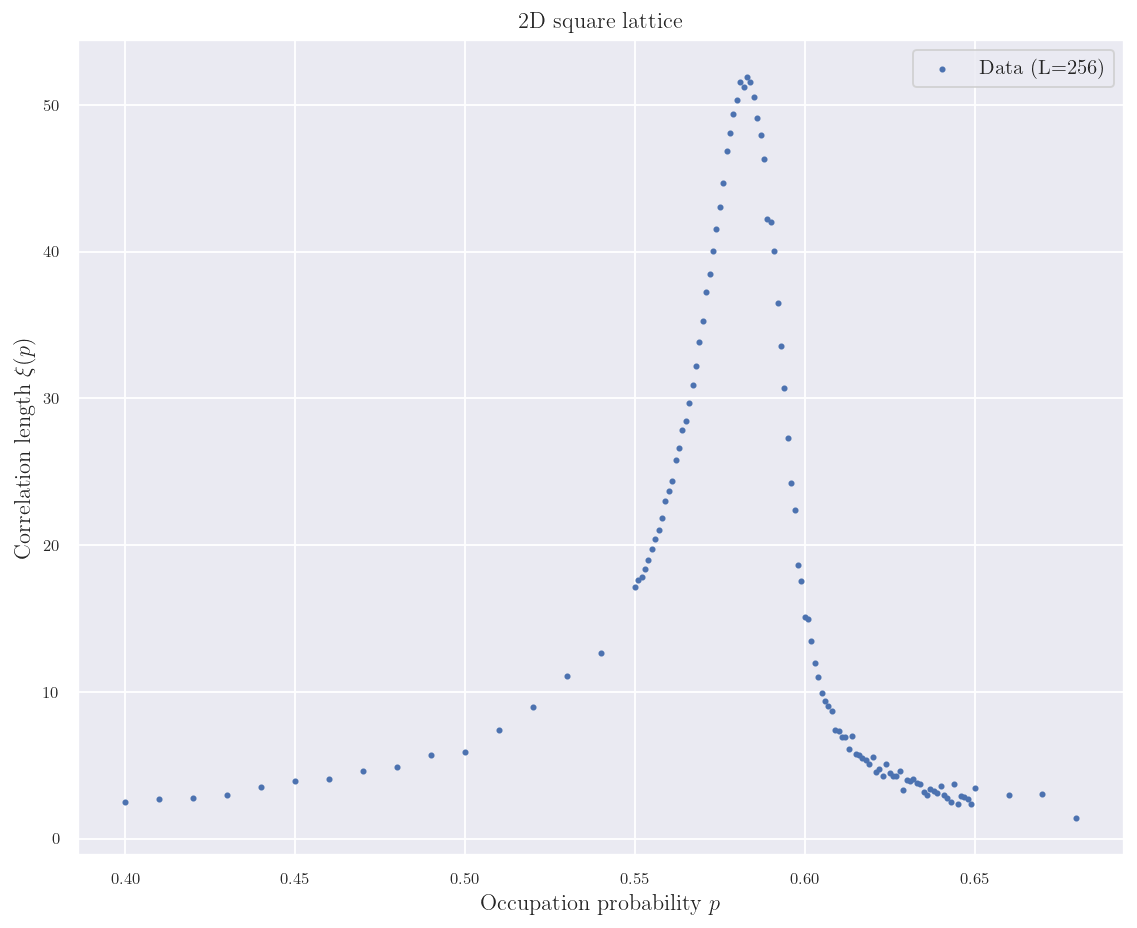
\includegraphics[width=\linewidth]{Images/sec3_corr_length_1.png}
  \caption{Correlation length for multiple lattice sizes}
  \label{fig:sec3_corr_length_1}
\end{figure}




% In 2D percolation, it is normally assumed that $g(r)$ behaves as the product of a power function and a exponential function(REF4), i.e 


\clearpage
